\section{Vektoren}

Ein Vektor beschreibt eine Verscheibung mit Richtung im Raum.
Ein Vektor kann von jedem Ort im Raum ausgehen und kann dann einen Start- und Endpunkt haben.
Jeder Punkt im Raum lässt sich mit einem Vektor vom Ursprung $O$ zu den
Koordinaten des Punktes beschreiben.

\begin{equation*}
    \vec{v} = \begin{bmatrix}
        5 \\
        3 \\
        7
    \end{bmatrix}
    \qquad A (1, 2, 2) \; B (4, 3, 1) \rightarrow \vec{AB} = \begin{bmatrix}
        3 \\
        1 \\
        -1
    \end{bmatrix}
    \qquad P (1, 3, 2) \rightarrow \vec{OP} = \begin{bmatrix}
        1 \\
        3 \\
        2
    \end{bmatrix}
\end{equation*}

\subsection{Rechnen mit Vektoren}

\subsubsection{Addition und Subtraktion}

Bei beim Rechnen mit Vektoren werden die Komponenten des einen Vektors
mit den Komponenten des anderen Vektors addiert bzw. subtrahiert.
Multiplikation ist dabei auf verschiedene Arten (später erklärt) möglich.
Division ist nicht möglich.

\begin{equation*}
    \begin{bmatrix}
        3 \\
        1 \\
        -2
    \end{bmatrix}
    +
    \begin{bmatrix}
        2 \\
        3 \\
        1
    \end{bmatrix}
    =
    \begin{bmatrix}
        5 \\
        4 \\
        -1
    \end{bmatrix}
    \qquad
    \begin{bmatrix}
        3 \\
        1 \\
        -2
    \end{bmatrix}
    -
    \begin{bmatrix}
        2 \\
        3 \\
        1
    \end{bmatrix}
    =
    \begin{bmatrix}
        1 \\
        -2 \\
        -3
    \end{bmatrix}
\end{equation*}

\subsubsection{Länge eines Vektor}

Die Länge eines Vektors ergibt sich aus dem Satz des Pythagoras.
Betragsstriche um einen Vektor bedeuten, dass dessen Länge gemeint ist.

\begin{equation*}
    \vec{AB} = \begin{bmatrix}
        3 \\
        1 \\
        -1
    \end{bmatrix}
    \qquad | \vec{AB} | = \sqrt{3^2 + 1^2 + (-1)^2} = \sqrt{11}
\end{equation*}

\subsubsection{Gegenvektor}

Der Gegenvektor ist die Umkehrung eines Vektors.

\begin{equation*}
    \vec{v} =
    \begin{bmatrix}
        3 \\
        -1 \\
        2
    \end{bmatrix}
    \qquad \vec{v} \cdot -1 = \vec{g} =
    \begin{bmatrix}
        -3 \\
        1 \\
        -2
    \end{bmatrix}
\end{equation*}

\subsubsection{Vektoren mit Vorfaktor}

Hat ein Vektor einen Vorfaktor (Skalar), so ist jede Komponente
des Vektors mit diesem zu multiplizieren.

\begin{equation*}
    2 \cdot
    \begin{bmatrix}
        3 \\
        -1 \\
        2
    \end{bmatrix}
    =
    \begin{bmatrix}
        6 \\
        -2 \\
        4
    \end{bmatrix}
\end{equation*}

\subsection{Kollineare Vektoren}

Vektoren sind kollinear, wenn sich der eine Vektor aus der Multiplikation
des anderen Vektors mit einem Skalar ergibt.
Sind zwei Vektoren kollinear, so bedeutet dies, dass beide die gleiche
Richtung beschreiben.

\begin{equation*}
    \vec{a} =
    \begin{bmatrix}
        4 \\
        6 \\
        2
    \end{bmatrix}
    \qquad
    \vec{b} =
    \begin{bmatrix}
        2 \\
        3 \\
        1
    \end{bmatrix}
    \qquad
    \vec{a} =
    2 \cdot \vec{b} =
    2 \cdot
    \begin{bmatrix}
        2 \\
        3 \\
        1
    \end{bmatrix}
    =
    \begin{bmatrix}
        4 \\
        6 \\
        2
    \end{bmatrix}
\end{equation*}

\subsection{Abstand von Punkten}

Um die Distanz zwischen zwei Punkten bzw. den Endpunkten von 2 vom gleichen Ort
ausgehenden Vektoren zu berechnen, muss nur die Länge des Differenzvektors berechnet
werden. Die Länge von $\vec{d}$ ist somit der Abstand zwischen
$\vec{v_1}$ und $\vec{v_2}$.
Eine Formel lässt sich somit von der Längenformel eines Vektors ableiten.

\begin{equation*}
    \vec{v_1} =
    \begin{bmatrix}
        4 \\
        6 \\
        2
    \end{bmatrix}
    \quad
    \vec{v_2} =
    \begin{bmatrix}
        1 \\
        2 \\
        0
    \end{bmatrix}
    \quad
    \vec{d} =
    \begin{bmatrix}
        3 \\
        4 \\
        2
    \end{bmatrix}
    \quad
    \begin{aligned}
        | \vec{d} | & = \sqrt{(x_1 - x_2)^2 + (y_1 - y_2)^2 + (z_1 - z_2)^2} \\
        | \vec{d} | & = \sqrt{(4 - 1)^2 + (6 - 2)^2 + (2 - 0)^2}
    \end{aligned}
\end{equation*}

\subsection{Mittelpunkt einer Strecke}

\subsection{Skalarprodukt}

Das Skalarprodukt ist die Summe der Produkte der einzelnen Vektorelemente.
Das Ergebnis ist eine relle Zahl.

\begin{equation*}
    \begin{bmatrix}
        3 \\
        1 \\
        -1
    \end{bmatrix} \cdot
    \begin{bmatrix}
        2 \\
        0 \\
        -1
    \end{bmatrix} = 3 \cdot 2 + 1 \cdot 0 + -1 \cdot -1 = 7
\end{equation*}

\subsubsection{Winkel beim Skalarprodukt}

Für den Winkel zwischen 2 vom gleichen Punkt ausgehenden Vektoren gelten folgende Formeln
Ist das Skalarprodukt gleich 0, so sind die Vektoren orthogonal, ist dass Skalarprodukt
gleich des Produkts der Vektorlängen, so sind die Vektoren kollinear.

\begin{equation*}
    \cos (\alpha) = \frac{\vec{a} \cdot \vec{b}}{|\vec{a}| \cdot |\vec{b}|}
    \qquad \vec{a} \cdot \vec{b} = 0 \Rightarrow \alpha = 90°
    \qquad \vec{a} \cdot \vec{b} = |\vec{a}| \cdot |\vec{b}| \Rightarrow \alpha = 0°
\end{equation*}

\subsubsection{Skalarprodukt: Assoziativ, Kommutativ und Distributiv}

Beim Skalarprodukt gelten die Rechengesetze Assoziativgesetz, Kommutativgesetz und Distributivgesetz.

\begin{equation*}
    \vec{a} \cdot \vec{b} = \vec{b} \cdot \vec{a}
    \qquad (\vec{a} \cdot \vec{b}) \cdot \vec{c} = \vec{a} \cdot (\vec{b} \cdot \vec{c})
    \qquad (\vec{a} + \vec{b}) \cdot \vec{c}  = \vec{a} \cdot \vec{c} + \vec{b} \cdot \vec{c} 
\end{equation*}

\subsection{Kreuzprodukt}

Das Kreuzprodukt zweier Vektoren ergibt einen dritten Vektor der orthogonal
zu beiden anderen ist. Das Kreuzprodukt von Rot-Blau ist der Vektor Pink, orthogonal zur
Ebene von Rot-Blau.

\begin{equation*}
    \vec{a} \times \vec{b} =
    \begin{bmatrix}
        a_1 \\
        a_2 \\
        a_3
    \end{bmatrix} \times
    \begin{bmatrix}
        b_1 \\
        b_2 \\
        b_3
    \end{bmatrix} =
    \begin{bmatrix}
        a_2 b_3 - a_3 b_2 \\
        a_3 b_1 - a_1 b_3 \\
        a_1 b_2 - a_2 b_1
    \end{bmatrix}
    \qquad
    \begin{bmatrix}
        3 \\
        1 \\
        -1
    \end{bmatrix} \times
    \begin{bmatrix}
        2 \\
        0 \\
        -1
    \end{bmatrix} =
    \begin{bmatrix}
        1 \cdot (-1) - (-1) \cdot 0 \\
        (-1) \cdot 2 - 3 \cdot (-1) \\
        3 \cdot 0 - 1 \cdot 2
    \end{bmatrix} =
    \begin{bmatrix}
        -1 \\
        1 \\
        -2
    \end{bmatrix}
\end{equation*}

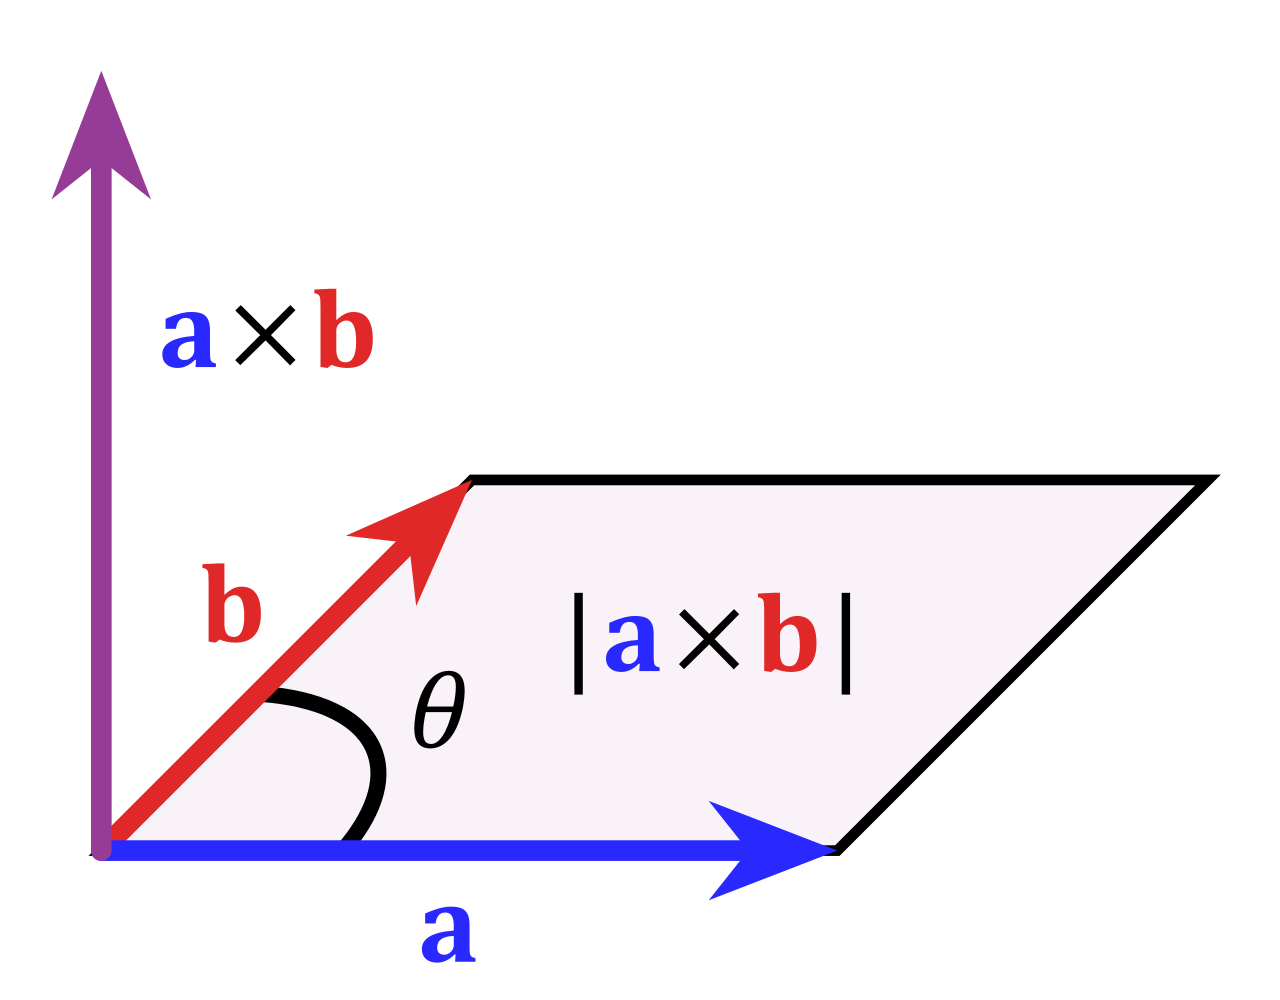
\includegraphics[width=0.4\textwidth]{images/cross-p.png}

\clearpage

\section{3D Koordinatensystem}

Die Darstellung eines 3D-Koordinatensystems in 2D (z. B. als Zeichnung auf Papier)
ist mit verschiedenen Abmessungen möglich. Außerdem ist es beim Punkte einzeichnen nötig,
strikt die Reihenfolge x, y, z einzuhalten.
Beim Ablesen von Punkten muss 1 Koordinate des Punktes bereits bekannt sein, da die Punkte
sonst mehrdeutig sind. Diese Angabe ist allerdings nicht immer explizit gegeben,
sondern ergibt sich meist aus dem Zusammenhang (z. B. von einer Aufgabe).

\begin{figure}[H]
    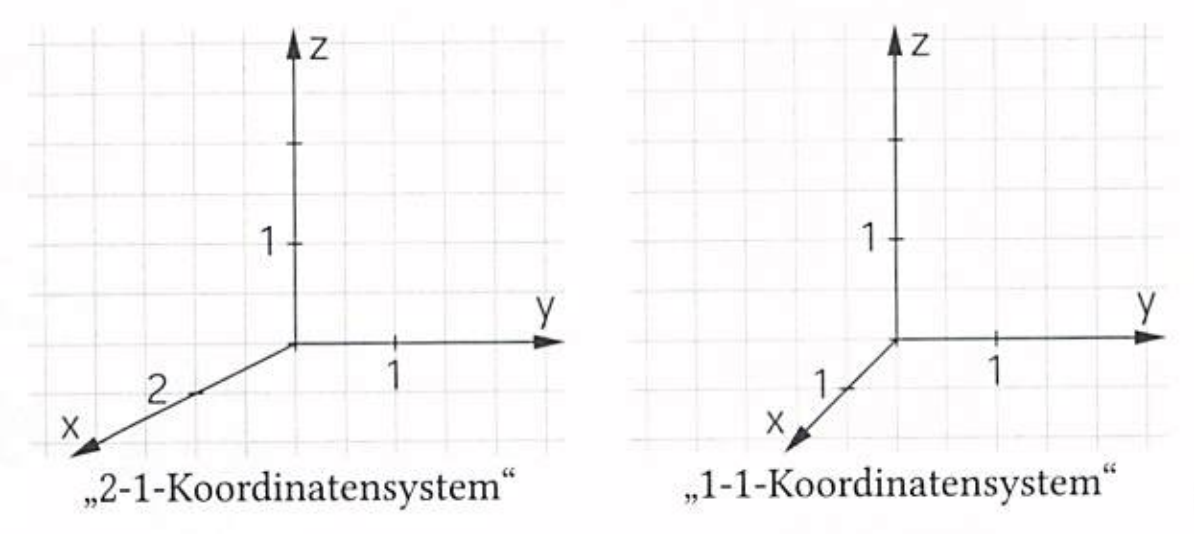
\includegraphics[width=0.8\textwidth]{images/3d-cord-systems.png}
    \caption{3D Koordinatensystem Arten}
\end{figure}

\begin{figure}[H]
    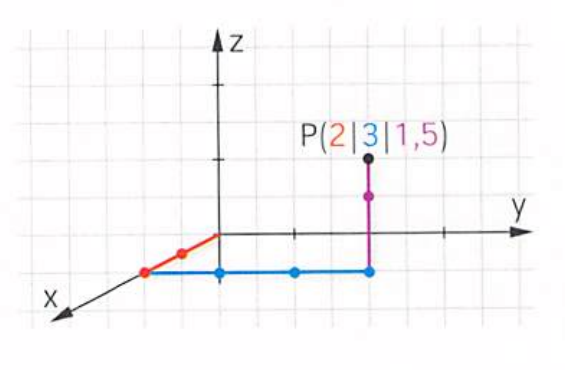
\includegraphics[width=0.6\textwidth]{images/3d-draw-point.png}
    \caption{Einzeichen von P(2 | 3 | 1,5)}
\end{figure}

\clearpage

\section{Geraden}

\subsection{Geradengleichung}

Eine Gerade im 3-dimensionalen Raum ist vergleichbar mit einer linearen Funktion im einem 2-dimensionalen
Koordinatensystem. Bei einer Gerade gibt es einen Startpunkt (vgl. y-Achsenabschnitt)
und eine Richtung (vgl. Steigung). Der Startpunkt wird Stützvektor genannt und beschreibt einen
Punkt im Raum. Die Richtung wird vom Richtungsvektor beschrieben. Da die Gerade im Raum
liegt, bestehen alle Koordinaten aus 3 Werten (also x, y, z).

\begin{equation*}
    g: \vec{x} = \vec{a} + r \cdot \vec{v}
    \qquad g: \vec{x} =
    \begin{bmatrix}
        2 \\
        1 \\
        3
    \end{bmatrix}
    +
    r \cdot
    \begin{bmatrix}
        1 \\
        1 \\
        2
    \end{bmatrix}
\end{equation*}

Eine Geradengleichung lässt sich aus 2 Punkten aufstellen. Einer der Punkte wird der
Stützvektor und der Richtungsvektor der Geraden ist der Differenzvektor der beiden Punkte.
Eine Gerade durch die Vektoren (Punkte) $\vec{c}$ und $\vec{d}$ wäre wie folgt.

\begin{equation*}
    \begin{aligned}
        \vec{a} & = \vec{c} \\
        \vec{v} & = \vec{c} - \vec{d}
    \end{aligned}
    \qquad g: \vec{x} = \vec{a} + r \cdot \vec{v}
\end{equation*}

Eine Gerade kann dabei durch Unendlich viele unterschiedliche Geradengleichungen
beschrieben werden, da jeder Punkt auf der Gerade als Stützvektor dienen kann
und da alle zum Richtungsvektor kollinearen Vektoren auch die gleiche Gerade
beschreiben.

\subsection{Spurpunkte auf Koordinatenebenen}

Eine Gerade kann 1, 2 oder 3 der Koordinatenebenen jeweils in einem Punkt schneiden.
Diese Punkte nennt man dann Spurpunkte. Ob eine Gerade eine bestimmte Koordinatenebene
schneidet lässt sich dadurch feststellen, dass für einen Wert $r$ die nicht zur Ebene
gehörende Koordinate gleich 0 ist. Eine Schnittpunkt einer Gerade in $P(10 | 0 | 10)$ würde
einen Spurpunkt auf der x-z Ebene bedeuten, da die y Koordinate gleich 0 ist.

\vspace*{0.2cm}

Für eine Gerade $g$ lässt sich z. B. der Spurpunkt der y-z Ebene bestimmten.
Die zu erfüllende Bedingung ist $x = 0$, die anderen Koordinaten sind egal.
Durch dass Komponentenweise gleichsetzen von Vektor und Geradengleichung lässt
sich, wenn es einen Spurpunkt gibt, der Wert von $r$ bestimmen, wenn dies der Fall ist.
Dazu muss die Gleichung der der auf 0 gesetzten Koordinate gelöst werden. 

\begin{equation*}
    g: \vec{x} =
    \begin{bmatrix}
        2 \\
        1 \\
        3
    \end{bmatrix}
    +
    r \cdot
    \begin{bmatrix}
        1 \\
        1 \\
        2
    \end{bmatrix}
    \qquad
    \begin{bmatrix}
        0 \\
        y \\
        z
    \end{bmatrix}
    =
    \begin{bmatrix}
        2 \\
        1 \\
        3
    \end{bmatrix}
    +
    r \cdot
    \begin{bmatrix}
        1 \\
        1 \\
        2
    \end{bmatrix}
    \qquad
    \begin{aligned}
        0 = 2 + r \cdot 1 \\
        \Rightarrow r = -2
    \end{aligned}
    \qquad
    \vec{s} =
    \begin{bmatrix}
        0 \\
        -1 \\
        -1
    \end{bmatrix}
\end{equation*}

\subsection{Lagebeziehungen von Geraden}
\subsubsection*{Geraden liegen parralel}

Die Geraden liegen parallel, wenn die Richtungsvektoren kollinear sind.

\subsubsection*{Geraden sind identisch}

Die Geraden sind identisch, wenn die Richtungsvektoren kollinear sind und
der Stützvektor der 1. Geraden auf der 2. Gerade liegt.
Dies lässt sich durch gleichsetzen von Stützvektor und Geradengleichung prüfen.

\subsubsection*{Geraden schneiden sich}

Die Geraden schneiden sich, wenn die Richtungsvektoren nicht kollinear sind
und für ein Wertepaar $r_1, r_2$ (Faktoren der Geradengleichungen) die Geradengleichungen
den gleichen Punkt beschreiben. Dies lässt sich durch gleichsetzen von 2 Geradengleichungen
überprüfen (Sind die Geraden identisch, so gibt es unendlich viele Wertepaare).
Daraus entsteht dann ein Gleichungssystem, was sich mit Hilfsmitteln (Taschenrechner)
oder von Hand lösen lässt.

\begin{align*}
    \vec{p} + r_1 \cdot \vec{u} = \vec{q} + r_2 \cdot \vec{v} \Rightarrow \\
    \\
    p_1 + r_1 \cdot u_1 = q_1 + r_2 \cdot v_1 \\
    p_2 + r_1 \cdot u_2 = q_2 + r_2 \cdot v_2 \\
    p_3 + r_1 \cdot u_3 = q_3 + r_2 \cdot v_3 \\
\end{align*}

\subsubsection*{Geraden liegen windschief}

Um zu überprüfen, ob die Geraden windschief liegen, muss versucht werden, ein Schnittpunkt
zu berechnen. Ergibt sich kein Schnittpunkt, so liegen die Geraden windschief.

\section{Ebenen}

Ein im Raum liegende Ebene lässt sich durch 3 nicht auf einer Gerade liegende Punkte
beschreiben. Folglich lässt sich somit auch aus 3 passenden Punkte eine Ebene konstruieren.
Eine Ebene wird dabei durch eine Ebenengleichung in Parameter-, Normalen- oder Koordinatenform
festgelegt.

\subsection{Ebenenformen}

\subsubsection{Parameterform}

Für 3 Vektoren (Punkte) lässt sich die Ebenengleichung in Parameterform wie folgt aufstellen.
Die Ebenengleichung in Parameterform besteht dabei aus einem Stützvektor und 2 Richtungsvektoren.
Alle Punkte im Raum, die bei einem Wertepaar r, s die Ebenengleichung erfüllen, liegen
dann auf der Ebene. Somit lässt sich für jeden Punkt im Raum bestimmen, ob dieser auf
der Ebene liegt.

\begin{align*}
    & E: \vec{s} + r \cdot \vec{v_1} + s \cdot \vec{v_2} \\
    \\
    & E: \vec{x} =
    \begin{bmatrix}
        3 \\
        7 \\
        4
    \end{bmatrix}
    +
    r \cdot
    \begin{bmatrix}
        0 \\
        2 \\
        -1
    \end{bmatrix}
    +
    s \cdot
    \begin{bmatrix}
        7 \\
        -3 \\
        5
    \end{bmatrix}
\end{align*}

\subsubsection{Normalenform}

Ein zu einer Ebene orthogonaler Vektor (orthogonal zu beiden Vektoren aus der Parameterform)
steht senkrecht auf dieser und ist der Normalenvektor dieser Ebene.
Bei der Normalenform ist $\vec{n}$ der Normalenvektor der Ebene und $\vec{q}$ ein Punkt
auf der Ebene. Wenn ein Punkt auf der Ebene liegt, so liegt auch der Differenzvektor von
diesem Punkt $\vec{x}$ und $\vec{q}$ in der Ebene. Somit ist dieser Differenzvektor dann
orthogonal zum Normalenvektor der Ebene. Alle Punkte, die nicht dieses Kriterium erfüllen,
liegen nicht auf der Ebene (vgl. Skalarprodukt ist 0, wenn Vektoren orthogonal).
Die Normalenform kann auch durch Ausmultiplizieren und Addieren des rechten Terms
Umgeformt werden, um eine andere Darstellung zu erhalten.

\begin{equation*}
    E: \vec{n} \cdot (\vec{x} - \vec{q}) = 0;
    E: \vec {n} \cdot \vec{x} = d = \vec{n} \cdot \vec{q}
\end{equation*}

\subsubsection{Koordinatenform}

Die Koordinatenform lässt sich aus der Normalenform umformen.
Jeder Punkt x, y, z der diese Gleichung erfüllt, liegt auf der Ebene.
Die Vorfaktoren für x, y, z sind dabei die Werte des Normalenvektors der Ebene.

\begin{align*}
    & E: \vec {n} \cdot \vec{x} = d = \vec{n} \cdot \vec{q} \\
    & E: n_1 \cdot x + n_2 \cdot y + n_3 \cdot z = d
\end{align*}

\subsubsection{Umwandlung zwischen den Formen}

\subsubsection*{Parameterform zu Normalenform}

Das Kreuzprodukt der beiden Richtungsvektoren ist der Normalenvektor.
Der Stützvektor fungiert als Punkt in der Ebene.

\subsubsection*{Normalenform zu Koordinatenform}

Im rechten und linken Term das Skalarprodukt ausrechnen.

\begin{equation*}
    E: \vec {n} \cdot \vec{x} = \vec{n} \cdot \vec{q}
\end{equation*}

\subsubsection*{Koordinatenform zu Normalenform}

Normalenvektor ablesen und einen Punkt bestimmen. Anschließend
Normalenform bilden.

\subsubsection*{Koordinatenform zu Parameterform}

Es müssen 3 Punkte bestimmt werden. Dabei ist es wichtig, dass diese nicht auf einer Gerade
liegen, da sonst die Parameterform nicht funktioniert. Aus diesen Punkten lassen sich
dann Stützvektor und Differenzvektoren bilden.

\subsection{Lagebeziehung Gerade-Ebene}

Liegt die Ebenengleichung in Koordinatenform vor (oder wird umgeformt), so lässt
sich die Geradengleichung Komponentenweise einsetzen. Anschließend lässt sich diese Gleichung
nach r umformen. Über r und die Geradengleichung lässt sich dann ein (potenzieller)
Schnittpunkt berechnen.
Gibt es keine Lösung für r, so liegen Gerade und Ebene parallel.
Gibt es 1 Lösung, so schneidet die Gerade die Ebene.
Gibt es $\infty$ Lösungen, so liegt die Gerade in der Ebene.

\begin{align*}
    & g: \vec{x} = \vec{a} + r \cdot \vec{v}
    \qquad E: n_1 \cdot x + n_2 \cdot y + n_3 \cdot z = d \\
    \\
    & n_1 \cdot (a_1 + r \cdot v_1) + n_2 \cdot (a_2 + r \cdot v_2) + n_3 \cdot (a_3 + r \cdot v_3) = d
\end{align*}

\subsection{Lagebeziehung Ebene-Ebene}

Vergleich mit der Gerade-Ebene beziehung lässt sich eine Ebenengleichung in Parameterform
in eine in Koordinatenform einsetzen.
Gibt es keine Lösung, so sind die Ebenen parallel.
Gibt es eine Abhängigkeit von r und s, so gibt es eine Schnittgerade.
Gibt es keine Abhängigkeit und $\infty$ Lösungen für r und s, so sind die Ebenen
identisch (liegen ineinander).

\begin{align*}
    & E: \vec{x} = \vec{a} + r \cdot \vec{u} + s \cdot \vec{v}
    \qquad E: n_1 \cdot x + n_2 \cdot y + n_3 \cdot z = d \\
    \\
    & n_1 \cdot (a_1 + r \cdot u_1 + s \cdot v_1) + n_2 \cdot (a_2 + r \cdot u_2 + s \cdot v_2) + n_3 \cdot (a_2 + r \cdot u_2 + s \cdot v_2) = d
\end{align*}

Wenn beide Ebenen in Koordinatenform vorliegen, so kann dies als Lineares-Gleichungssystem
gedeutet werd. Dass es 3 Variablen und 2 Gleichungen gibt ist in diesem Fall kein Problem,
da man eine Variable frei bestimmen darf. Anschließend lässt sich das lineare Gleichungssystem
lösen. Von den Unbekannten x, y, z wählt man für eine frei einen Wert und löst anschließnd
das System.
Gibt es keine Lösung, so sind die Ebenen parallel.
Gibt es eine Abhängigkeit von 2 Koordinaten, so gibt es eine Schnittgerade.
Gibt es keine Abhängigkeit und $\infty$ Lösungen die 2 Koordinaten, so sind die Ebenen
identisch (liegen ineinander).

\begin{align*}
    & E: n_{1.1} \cdot x + n_{1.2} \cdot y + n_{1.3} \cdot z = d_1 \\
    & E: n_{2.1} \cdot x + n_{2.2} \cdot y + n_{2.3} \cdot z = d_2
\end{align*}

\clearpage

\subsection{Winkel zwischen Geraden und Ebenen}

Der Winkel zwischen 2 im gleichen Punkt startenden Vektoren lässt sich mit dem
Skalarprodukt bestimmen. Dabei ist es wichtig, die richtigen Richtungsvektoren
zu wählen, die im gleichen Punkt beginnen.
Außerdem ist es wichtig, ob der Winkel oder der Gegenwinkel gesucht ist.
Beide ergänzen sich zu 180° und sind voneinander abhängig.

\begin{align*}
    & \cos (\alpha) = \frac{\vec{a} \cdot \vec{b}}{|\vec{a}| \cdot |\vec{b}|} \\
    & \beta = 180° - \alpha
\end{align*}

\subsubsection*{Winkel Gerade-Gerade}

Einer der Winkel zwischen den beiden Richtungsvektoren muss berechnet werden.

\subsubsection*{Winkel Gerade-Ebene}

Einer der Winkel zwischen dem Richtungsvektor und dem Normalenvektor muss berechnet werden.

\subsubsection*{Winkel Ebene-Ebene}

Einer der Winkel zwischen den beiden Normalenvektoren muss berechnet werden.

\subsection{Abstände im Raum}

\subsubsection{Abstand Punkt-Gerade}

Wenn $\vec{f}$ der Punkt auf der Gerade mit dem geringsten Abstand zu $\vec{p}$ ist,
gilt dass $\vec{f}$ der Lotfußpunkt ist und der Diffrenzvektor von $\vec{f}$ und $\vec{p}$
orthogonal zum Richtungsvektor $\vec{v}$ der Geraden ist. Daraus ergibt sich folgende
Formel, um den Punkt $\vec{f}$ zu berechnen. Die Länge des Differenzvektors von $\vec{f}$,
$\vec{p}$ ist dann die kürzeste Distanz zwischen Gerade und Punkt.

\begin{equation*}
    (\vec{p} - \vec{f}) \cdot \vec{v} = 0
    \qquad |\vec{p} - \vec{f}| = d
\end{equation*}

Ein weitere Möglichkeit ist die Bestimmung über die Analysis. Es kann dass Minimum
einer Funktion der Distanz $d(r) = |\vec{f}(r) - \vec{p}|$ bestimmt werden,
sodass man den $r$ Wert herausfindet.
$\vec{f}(r)$ beschreibt dabei einen Punkt auf der Gerade, der von $r$ abhängig ist.

\subsubsection{Abstand Punkt-Ebene}

Zur Bestimmung vom Abstand eines Punktes zu einer Ebene, muss zuerst
eine Lotgerade gebildet werden. Der Stützvektor ist der Punkt $\vec{p}$
und der Richtungsvektor ist der Normalenvektor $\vec{n}$ der Ebene.
Anschließend lässt sich ein Schnittpunkt dieser Lotgerade und der Ebene
bestimmen, der Lotfußpunkt $F$. Die Distanz zwischen $\vec{p}$ und $F$ ist
die kürzeste Distanz zwischen Punkt und Ebene.

\begin{center}
    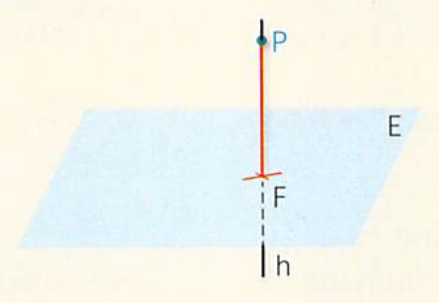
\includegraphics[width=0.4\textwidth]{images/3d-point-plane-distance.png}
\end{center}

\subsubsection{Abstand windschiefer Geraden}

Bei 2 windschiefen Geraden ist die Distanz zwischen zwei Punkten $P$ und $Q$,
jeweils 1 auf jeder Gerade, dann am geringsten, wenn der Diffrenzvektor von $P$ und $Q$
orthogonal zu beiden Richtungsvektoren ist. P ist dabei Abhängig von $s$ und $Q$ von $r$.
Dieses Lineare-Gleichungssystem lässt sich nun lösen (2 Variablen, 2 Gleichungen).

\begin{align*}
    & (\vec{P} - \vec{Q}) \cdot \vec{u} = 0 \\
    & (\vec{P} - \vec{Q}) \cdot \vec{v} = 0 \\
    \\
    & (\vec{P}(s) - \vec{Q}(r)) \cdot \vec{u} = 0 \\
    & (\vec{P}(s) - \vec{Q}(r)) \cdot \vec{v} = 0
\end{align*}

\clearpage

\subsubsection{Abstände bei parallelen Geraden und Ebenen}

Ist der Abstand bei parallelen Ebenen, Geraden oder Kombinationen gesucht,
so lässt sich einfach auf einer ein Punkt bestimmen und dann der kürzeste Abstand
dieses Punktes zum anderen Objekt berechnet werden.

\begin{center}
    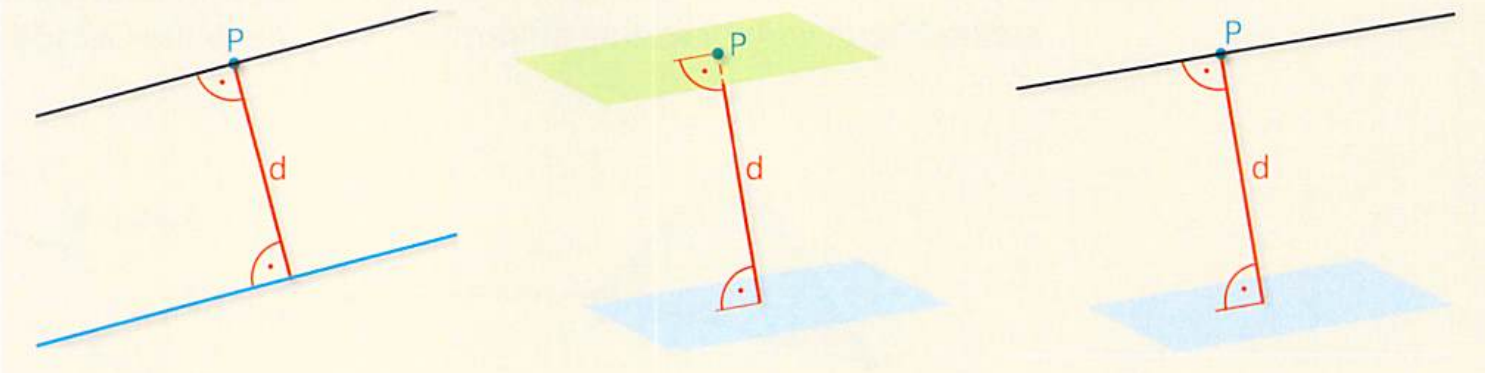
\includegraphics[width=1.0\textwidth]{images/3d-parallel-distance.png}
\end{center}

\section{Spiegelungen}

\subsection{2D Spiegelungen}

Achsenspiegelung und Punktspiegelung im 2-dimensionalen Raum.

\begin{figure}[H]
    \adjustbox{scale=0.8}{
    \begin{tikzpicture}
        % system
        \tkzInit[xmin=-4,xmax=4,ymin=-4,ymax=4]
        \tkzGrid
        \draw [thick,->] (-4.5, 0) -- (4.5, 0);
        \draw [thick,->] (0, -4.5) -- (0, 4.5);
        \node at (4.5, -0.5) {x};
        \node at (-0.5, 4.5) {y};
        % vectors, points
        \draw[red, arrows = {-Stealth}] (0, 2) -- (2.9, 2);
        \draw[red, arrows = {-Stealth}] (0, 2) -- (-2.9, 2);
        \draw[blue] (0, -4) -- (0, 4);
        \draw [color=blue, fill=green] (3, 2) circle (0.05);
        \draw [color=blue, fill=green] (-3, 2) circle (0.05);
    \end{tikzpicture}
    }
    \adjustbox{scale=0.8}{
    \begin{tikzpicture}
        % system
        \tkzInit[xmin=-4,xmax=4,ymin=-4,ymax=4]
        \tkzGrid
        \draw [thick,->] (-4.5, 0) -- (4.5, 0);
        \draw [thick,->] (0, -4.5) -- (0, 4.5);
        \node at (4.5, -0.5) {x};
        \node at (-0.5, 4.5) {y};
        % vectors, points
        \draw[red, arrows = {-Stealth}] (0, 0) -- (2.9, 2);
        \draw[red, arrows = {-Stealth}] (0, 0) -- (-2.9, -2);
        \draw [color=blue, fill=green] (3, 2) circle (0.05);
        \draw [color=blue, fill=green] (-3, -2) circle (0.05);
        \draw [color=blue, fill=blue] (0, 0) circle (0.1);
    \end{tikzpicture}
    }
\end{figure}

\subsection{3D Spiegelungen}

Punktspiegelung, Ebenenspiegelung und Achsenspiegelung im 3-dimensionalen Raum.

\begin{figure}[H]
    \centering
    \setkeys{Gin}{width=0.3\linewidth}
    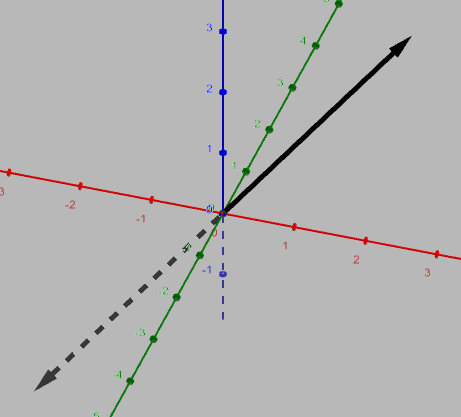
\includegraphics[width=0.3\textwidth]{images/3d-point-reflection.png} \,
    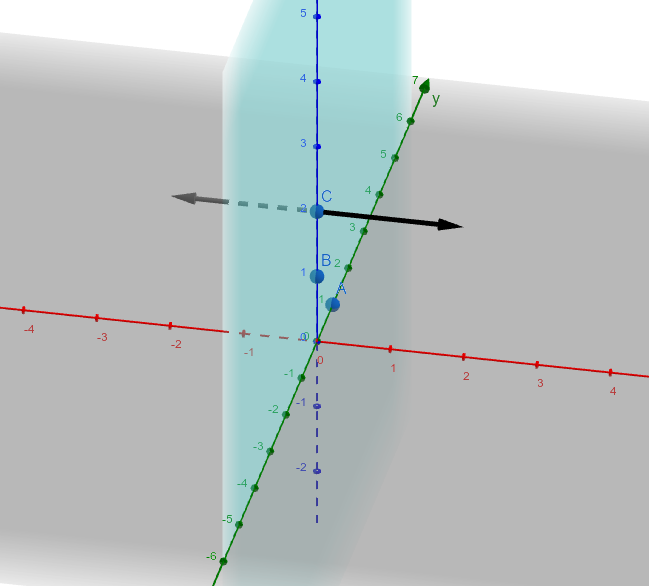
\includegraphics[width=0.3\textwidth]{images/3d-plane-reflection.png} \,
    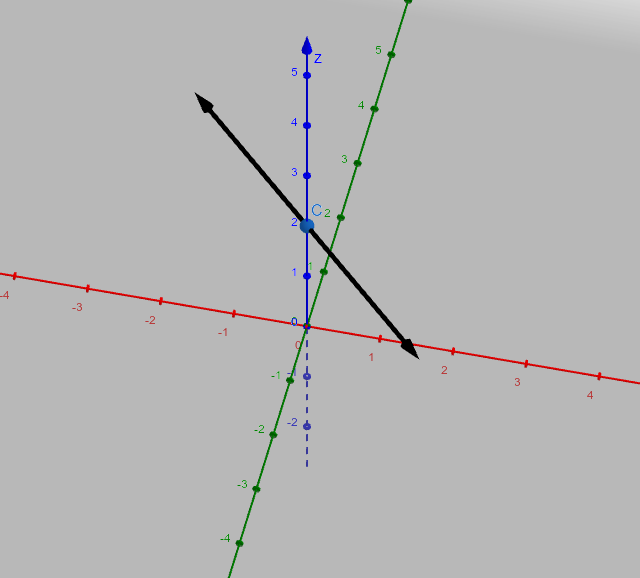
\includegraphics[width=0.3\textwidth]{images/3d-axis-reflection.png}
\end{figure}

\subsubsection{Punkspiegelung}
Für die Punktspiegelung muss für alle Punkte der Gegenvektor zum  Verbindungsvektor von
Spiegelpunkt und zu spiegelndem Punkt gebildet werden. Dieser zeigt dann vom Spiegelpunkt
aus gesehen zur neuen Position des Punktes.
Es verändern sich maximal alle 3 Koordinaten des Punktes.

\subsubsection{Ebenenspiegelung}
Um einen Punkt an einer Ebene zu spiegeln, muss man zuerst den Punkt auf der
Ebene mit dem geringsten Abstand (Lotpunkt) zu diesem bestimmen. Anschließend
spiegelt man den Punkt einfach anhand dieses Punktes. Alternativ kann dies
auch mit einer Geradengleichung (vgl. Lotgerade) realisiert werden.
Es verändert sich maximal 1 Koordinate des Punktes.

\subsubsection{Achsenspiegelung}
Um einen Punkt an einer Achse zu spiegeln, muss man zuerst den Punkt auf der
Achse mit dem geringsten Abstand zu diesem bestimmen (vgl. Punkt-Gerade Abstand).
Anschließend spiegelt man den Punkt einfach anhand dieses Punktes.
Es verändern sich maximal 2 Koordinaten des Punktes.
